\documentclass[10pt, conference]{IEEEtran}

% correct bad hyphenation here
%\hyphenation{op-tical net-works semi-conduc-tor}

\usepackage{url}
\usepackage{graphicx}
\usepackage{dcolumn}
\usepackage{color}

\newcommand{\nPrograms}{250,163}
\newcommand{\nAnalyzedPrograms}{247,798}
\newcommand{\nemptyPrograms}{14,307}
\newcommand{\nScriptPrograms}{233,491}
\newcommand{\nLOC}{36,085,654}
\newcommand{\nscripts}{4,049,356}


\newcommand{\fenia}[1]{\emph{\color{blue}Fenia says: #1}}
\newcommand{\felienne}[1]{\emph{\color{green}Felienne says: #1}}
\newcommand{\grex}[1]{\emph{\color{yellow}Gregorio says: #1}}
\newcommand{\jemole}[1]{\emph{\color{red}Jesús says: #1}}

\begin{document}

\title{A dataset of Scratch programs,\\Scraped, Shaped and Scored}


\author{
	\IEEEauthorblockN{Efthimia Aivaloglou\IEEEauthorrefmark{1}, Felienne Hermans\IEEEauthorrefmark{1}, Gregorio Robles\IEEEauthorrefmark{2}, and Jes{\'u}s Moreno-Le{\'o}n\IEEEauthorrefmark{3}}
	
	\IEEEauthorblockA{\IEEEauthorrefmark{1}Delft University of Technology, The Netherlands\\
			Email: \{e.aivaloglou, f.f.j.hermans\}@tudelft.nl}
	\IEEEauthorblockA{\IEEEauthorrefmark{2}Universidad Rey Juan Carlos, Fuenlabrada (Madrid), Spain \\
		Email: grex@gsyc.urjc.es}
	\IEEEauthorblockA{\IEEEauthorrefmark{3}Programamos.es \& Universidad Rey Juan Carlos, Spain\\
		Email: jesus.moreno@programamos.es}
}

\maketitle


\begin{abstract}
In this paper, we present a collection of 250K Scratch programs scraped from the Scratch project repository. We processed the program data to encode it into a database that facilitates querying and further analysis. The dataset is intended as an input for research on computing education and source code analysis.
\end{abstract}

\begin{IEEEkeywords}
Scratch; dataset;
\end{IEEEkeywords}


 
\section{Introduction}
Scratch \cite{resnick_scratch:_2009} is a block-based programming language developed to serve as a stepping stone for children from 8 to 16 years old to the more advanced world of computer programming.
It offers a web-based programing environment that enables creating games and interactive animations. The public repository of Scratch programs contains over 19 million projects and 16 million users.

A number of works in the computing education research field attempt to assess the programming skills that novice programmers develop in the Scratch environment.
Some utilize program data collected during specific programming courses (e.g., \cite{meerbaum-salant_learning_2010, wilson_evaluation_2012, Maloney_2008}), while others utilize the dataset made available by the Lifelong Kindergarten Group at the MIT Media Lab, which contains data for Scratch projects created until 2012 (e.g., \cite{fields_2014, yang_2015, Dasgupta_2016}).
In addition to identifying indications of learning of programming concepts, static analysis of Scratch programs has also been performed for identifying code smells and bad programming practices within Scratch programs \cite{Meerbaum_habits_2011, Aivaloglou_2016}, and automated quality assessment tools have been proposed (e.g. Hairball \cite{boe_hairball:_2013} and Dr. Scratch \cite{moreno_automatic_2014}).

While Scratch is receiving increasing interest as an introductory programming language, there is no recent dataset of Scratch programs available to the research community.
The one made available from the MIT Media Lab concerns projects created using the previous, initial version of the Scratch application, before the introduction of the Scratch 2 web programming interface in 2013.
It is since then that the popularity of Scratch started increasing\footnote{Monthly activity trends can be found at \url{https://scratch.mit.edu/statistics/}}.

The goal of this paper is to present an open and timely dataset of recent Scratch programs, along with their metadata, that can facilitate quantitative research in the fields of source code analysis and computing education.
The dataset contains 250 thousand Scratch projects, from more than 100 thousand different users, that were scraped from the Scratch project repository.
It is made available as a database\footnote{{\fenia{add anonymized address, update it in repo footnote}}} which includes, for each Scratch project, its metadata and the program data, along with programming mastery scoring results from the Dr. Scratch quality assessment tool \cite{moreno_automatic_2014}.

\section{Dataset Construction}
\label{dataset}

\subsection{Data collection}
To collect the data from the web interface of the Scratch project repository we built a scraping program.
The web scraping program, called Kragle, starts by reading the Scratch projects page\footnote{\label{scratchpublic}\url{https://scratch.mit.edu/explore/projects/all/}} and thus obtains the project identifiers of projects that were most recently shared.
Subsequently, Kragle retrieves the JSON code for each of the listed projects\footnote{For a given project id $x$, the program's JSON representation can be obtained via \url{https://cdn.projects.scratch.mit.edu/internalapi/project/x/get}}.

We ran Kragle on March 2nd 2016 for 24 hours and, during that time, it obtained the JSON code for \nPrograms projects. Out of those, we failed to parse and further analyze 2,367 projects due to technical difficulties with the JSON files.
Kragle, as well as all scraped projects and our analysis files are available.\footnote{\label{repo}\url{https://github.com/TUDelftScratchLab/ScratchDataset}}

Once we obtained the Scratch projects, we parsed the JSON files according to the specification of the format\footnote{\url{http://wiki.scratch.mit.edu/wiki/Scratch_File_Format_(2.0)}}.
This resulted in a list of used blocks per project, within the sprites and the stage of the project.
We also cross referenced all blocks with the Scratch wiki to determine the shapes and the category of all blocks.
For example, \texttt{When Green Flag Clicked} is a \emph{Hat block} from the \emph{Events category}.
We included the blocks from Scratch extensions, such as the LEGO WeDo extensions, that we found in the dataset.

\subsection{Calculation of programming mastery scores}
\fenia{Description of how the mastery metrics for       
	[Abstraction]
	,[Parallelism]
	,[Logic]
	,[Synchronization]
	,[FlowControl]
	,[UserInteractivity]
	,[DataRepresentation]
	,[Mastery]
	,[Clones]
	,[CustomBlocks]
	,[InstancesSprites]
	were calculated}

\subsection{Importing the data}
\label{dataAnalysis}
All scraped project data and metadata, including the list of used blocks and parameters, were imported in a relational database.
We also imported the data on the shapes and the categories of the Scratch blocks.
We then used SQL queries for normalizing the data and bringing it in its final schema, outlined in Table \ref{tbl-dbschema}.

\begin{table}[]
	\centering
	\begin{tabular}{llp{5.4cm}}
		\textbf{Table}& \textbf{Key} & \textbf{Attribute(Description)}\\
		\hline
		\textbf{\texttt{project}} & PK & \texttt{p\_id} (Scratch project ID)\\
		&  & 							\texttt{project-name} (name given to project)\\
		&  & 							\texttt{username} (author's Scratch 
		username)\\
		&  & 							\texttt{total-views} (project views number)\\
		&  & 							\texttt{total-remixes} (project remixes number)\\
		&  & 							\texttt{total-favorites} (total users favoriting)\\
		&  & 							\texttt{total-loves} (total users `loving' the project)\\
		& & 							\texttt{is-remix} (calculated column, true if project is a remix of another one)\\
		\hline
		\textbf{\texttt{script}} & PK & \texttt{script\_id} (auto increment)\\
		& FK & 							\texttt{project\_id} (\texttt{\scriptsize{*\ldots1 project:p\_id}})\\
		& & 							\texttt{sprite-type} (one of [sprite, stage, procDef])\\
		& & 							\texttt{sprite-name} (name sprite the script is in)\\
		& & 							\texttt{script-rank} (project-level ranking of script)\\
		& & 							\texttt{coordinates} (x-y location of script in Scratch editor)\\
		& & 							\texttt{total-blocks} (calculated column, number of blocks comprising the script)\\
		\hline
		\textbf{\texttt{procedure}} & PK,FK & \texttt{script\_id} (\texttt{\scriptsize{1\ldots1 script:script\_id}})\\
		& & 							\texttt{proc-name} (name given to custom block)\\
		& & 							\texttt{total-args} (number of input arguments)\\
		\hline
		\textbf{\texttt{block}} & PK,FK  & \texttt{script\_id} (\texttt{\scriptsize{*\ldots1 script:script\_id}})\\
		& PK & \texttt{block-rank} (script-level ranking of block)\\
		& FK & \texttt{block-type} (\texttt{\scriptsize{*\ldots1 blockType:b-type}})\\
		&  & \texttt{parameter-1} (value of 1st input parameter)\\
		&  &\vdots\\
		&  & \texttt{parameter-24} (value of 24th input parameter)\\
		\hline
		\textbf{\texttt{blockType}} & PK & \texttt{b-type} (Scratch name of predefined block)\\
		&  & \texttt{category} (Scratch block category)\\
		&  & \texttt{shape} (One of the 8 block shapes in the Scratch interface)\\
		&  & \texttt{is-input} (true if the block receives user input)\\
		\hline
		\textbf{\texttt{remix}} & PK  & \texttt{remix\_id} (\texttt{\scriptsize{project\_id}} of created project)\\
		&  & \texttt{from-project\_id} (\texttt{\scriptsize{project\_id}} of original project)\\
		\hline
		\textbf{\texttt{grades}} & PK,FK & \texttt{project\_id} (\texttt{\scriptsize{1\ldots1 project:p\_id}})\\
		& & \texttt{Abstraction} (\fenia{short descriptions})\\
		& & \texttt{Parallelism} ()\\
		& & \texttt{Logic} ()\\
		& & \texttt{Synchronization} ()\\
		& & \texttt{FlowControl} ()\\
		& & \texttt{UserInteractivity} ()\\
		& & \texttt{DataRepresentation} ()\\
		& & \texttt{Mastery} ()\\
		& & \texttt{Clones} ()\\
		& & \texttt{CustomBlocks} ()\\
		& & \texttt{InstancesSprites} ()\\
		\hline
	\end{tabular}
	\caption{Database schema: Tables and Attributes}
	\label{tbl-dbschema}
\end{table}

\section{Dataset Description}

\subsection{Data Representation}

The projects' data are stored in a relational database. Each \textbf{\texttt{project}} is identified by its Scratch project ID, stored in field \texttt{p\_id}, while its author is identified by the \texttt{username}\footnote{Each project and author page can be accessed in the Scratch web interface at \url{https://scratch.mit.edu/projects/<p_id>} and \url{https://scratch.mit.edu/users/<username>} respectively}.
If a project is a remix of another one, the original project can be found in the \textbf{\texttt{remix}} table.
Table \textbf{\texttt{grades}} stores the Dr. Scratch results for the programming mastery metrics per project.
 
 \begin{figure}
 	\centering
 	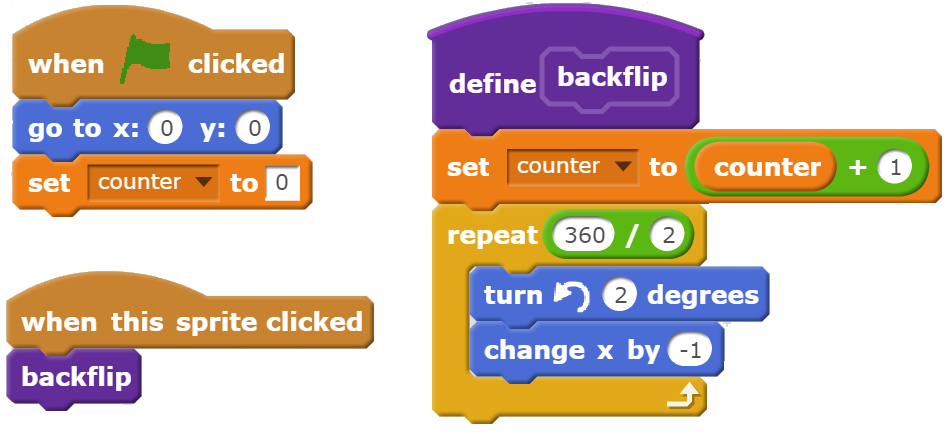
\includegraphics[width=0.45\textwidth]{scratchExample}
 	\caption{Example of a Scratch program with three scripts in the same spite}
 	\label{fig-scratchExample}
 \end{figure}

The schema of the database, outlined in Table \ref{tbl-dbschema}, reflects the structure of the Scratch programs.
Projects contain sprites, which are entities with their own associated code.
The code is organized into \textbf{\texttt{script}}s, i.e., groups of Scratch code blocks, each script belonging a sprite named \texttt{sprite-name}.
In the example in Figure \ref{fig-scratchExample} there are 3 scripts, one initiated when the green flag is clicked, one then the sprite is clicked, and the `backflip' custom block definition.
Those custom blocks are the equivalent of procedure definitions, with their names and arguments stored in the \textbf{\texttt{procedure}} table.

The coding elements in the Scratch environment are the \textbf{\texttt{block}}s, which can receive input parameters.
In the example in the figure, block `go to x:0 y:0' receives as input two numerical parameters.
Custom clock invocations are stored in this table just like regular blocks.
To cater for the varying number of input parameters that those blocks can have, this table can store up to the maximum number of input parameters found in the dataset, which is 24.
The ordering of the blocks in the scripts can be retrieved using the \texttt{block-rank} field, which represents a depth-first ranking of the blocks.
In the script of the `backflip' custom block definition in the example, the ranking of the blocks would be `define backflip', `set counter to', `+', `counter', followed by the rest of the blocks.
The clocks can be of different shapes and categories.
In table \textbf{\texttt{blockType}} we have stored the encoding of all types of Scratch blocks and the blocks from Scratch extensions.

\subsection{Dataset Contents}

\begin{table}[]
	\centering
	\begin{tabular}{lr}
		\hline
		Projects & 250,163 \\
		Non-empty projects & 233,491 \\
		Remixes of other projects & 12,167 \\
		Usernames & 109,960 \\
		Scripts & 4,049,356 \\
		Blocks & 36,085,654 \\
		Custom block definitions & 209,769 \\
		Projects analyzed by Dr. Scratch & 231,050 \\
		\hline
	\end{tabular}
	\caption{Dataset contents}
	\label{tbl-size}
\end{table}

\begin{table*}[]
	\centering
	\begin{tabular}{lrrrrrr}
		&\textbf{mean}&\textbf{min}&\textbf{Q1}&\textbf{median}&\textbf{Q3}&\textbf{max}\\
		\hline
		Projects per username&2.27&1&1&1&2&868\\
		Sprites per project&5.30&0&1&2&5&525\\
		Scripts per project&16.19&0&2&4&11&3,038\\
		Blocks per project&144.25&0&9&26&69&34,622\\
		Custom block definitions per project&0.64&0&0&0&0&372\\
		Total views per project&5.76&0&1&1&4&27,993\\
		Total remixes per project&197.12&0&0&0&0&14,951,164\\
		Total favorites per project&0.54&0&0&0&0&2,582\\
		Dr. Scratch mastery score per project&8.92&0&6&8&11&21\\
		\hline
	\end{tabular}
	\caption{Summary statistics of the dataset}
	\label{tbl-stats}
\end{table*}

As shown in Table \ref{tbl-size}, the dataset contains the metadata of 250,163 Scratch projects and the code of 233,491 of those that are non-empty.
The projects were created from 109,960 different users.
Most of those, as shown in Table \ref{tbl-stats}, have created a single project.
However, 40 thousand users have created more than one and up to 868 projects in the dataset.

The majority of the projects have been viewed only once, and they have not been favorited or remixed.
Around 10 thousand of the total projects have been remixed at least once, while the dataset includes cases of very popular projects with more than 100 remixes and even one thousand cases with more than 100 views. 

Table \ref{tbl-stats} also reveals the median project in the dataset: it contains 2 sprites, 4 scripts, 26 blocks, no custom block definitions, and receives a mastery score of 8 our of 21.
The table also highlights the existence of surprisingly complex projects, with 525 sprites, 3 thousand scripts as 34 thousand blocks.

\fenia{Should we add some stats about the Dr Scratch master scores?}

\section{Using the Dataset / Enabled Research / Research Opportunities}
a description of how the data has been used by others,

\section{Extending the Dataset}
ideas for what future research questions could be answered or what further improvements could be made to the data set

\section{Limitations}
any limitations and/or challenges in creating or using this data set.

\section{Conclusion}

\bibliographystyle{IEEEtran}
\bibliography{IEEEabrv,ScratchDataset}

\end{document}


